%%%%%%%%%%%%%%%%%%%%%%%%%%%%%%%%%%%%%
%									%
%	Copyright 2014 - Julian Nonino	%								
%									%
%%%%%%%%%%%%%%%%%%%%%%%%%%%%%%%%%%%%%

\documentclass[a4paper,12pt,openright,twoside]{article}

% Paquetes
	
	% Idioma y codificacion de caracteres
		\usepackage[spanish]{babel}
		\usepackage[latin1]{inputenc}
	
	% Figuras
		\usepackage{graphicx}
		\usepackage{subfigure}
		\usepackage{float} % Para posicionar imagenes donde uno quiera. Solo hay que poner la opcion [H]
	
	% Apendice
		\usepackage{appendix}
	
	%Tablas	
	%\usepackage{tabular}
	
	% Margenes
		\usepackage{anysize}
	
	% Matematica
		\usepackage[cmex10]{amsmath}
		\usepackage{amssymb}
	
	% Referencias
		\usepackage{hyperref}
		\usepackage[defernumbers=true, backend=bibtex]{biblatex}
		\DeclareBibliographyCategory{cited}
		\AtEveryCitekey{\addtocategory{cited}{\thefield{entrykey}}}
		\addbibresource{referencias.bib}
		\nocite{*}
	
	% Colores
		\usepackage{color}
		% Definicion de colores
			\definecolor{dkgreen}{rgb}{0,0.6,0}
			\definecolor{gray}{rgb}{0.5,0.5,0.5}
			\definecolor{mauve}{rgb}{0.58,0,0.82}
			\definecolor{violeta}{RGB}{127,0,85}

	% Margenes
	% {izquierda}{derecha}{arriba}{abajo}
		\marginsize{3cm}{3cm}{2.5cm}{2.5cm}

	% Encabezados
		\pagestyle{headings}
		
% Documento
\begin{document}
 
	% Reeescritura de comandos
		\renewcommand{\appendixname}{Ap�ndice}
		\renewcommand{\appendixtocname}{Ap�ndice}
		\renewcommand{\tablename}{\textbf{Tabla}} 	% Para poner la palabra en mayusucula
		\renewcommand{\figurename}{\textbf{Figura}} % Para poner la palabra en mayuscula
		\setcounter{secnumdepth}{3} % Para numerar subsubsecciones

	% Portada
 		\begin{titlepage}
 			%%%%%%%%%%%%%%%%%%%%%%%%%%%%%%%%%%%%%
%									%
%	Copyright 2014 - Julian Nonino	%								
%									%
%%%%%%%%%%%%%%%%%%%%%%%%%%%%%%%%%%%%%

% PAGINA ANTERIOR
	\vspace*{0.15in}

	\begin{center}		
	
		\begin{LARGE}
			\textbf{Plan de Trabajo para Tesis de Maestr�a}
		\end{LARGE}
		\vspace*{0.15cm}
		\rule{15cm}{0.1mm} 
		\vspace*{0.15cm}
		\begin{Large}Maestr�a en Ingenier�a en Sistemas de Informaci�n\end{Large}\\
	
		\vspace*{4cm}
	
		\begin{Huge}
			Juli�n Nonino
		\end{Huge}
		\\
		
		\vspace*{2cm}
		
		\begin{Large}
			Director
			\\
			\vspace*{0.5cm}
			Mart�n Miceli
		\end{Large}
		
		\vspace*{3.5cm}
		
		\begin{figure}[H]
			\centering
			
\includegraphics[width=.10\linewidth]{./portada/logo_utn}
		\end{figure}	
		
		\begin{large}Universidad Tecnol�gica Nacional\end{large}\\
		\vspace*{0.2cm}
		\begin{large}Facultad Regional C�rdoba\end{large}\\
		\vspace*{0.2cm}
		\begin{large}Direcci�n de Posgrado\end{large}\\
		\vspace*{1cm}
		C�rdoba\\
		- 2014 -
	\end{center}

% PAGINA POSTERIOR
	\newpage
	\mbox{}
	\thispagestyle{empty}
	
 			\thispagestyle{empty}
 		\end{titlepage}
 		
	% T�tulo
		\section{T�tulo de la Tesis}
		\label{sec:titulo}
		
		El t�tulo del la tesis de maestr�a ser�:
		
		\begin{quote}
			\textbf{\emph{Herramienta did�ctica basada en la nube para
			planeamiento y estimaci�n en Scrum.}}
		\end{quote}
			
	% Justificaci�n del tema elegido
		%%%%%%%%%%%%%%%%%%%%%%%%%%%%%%%%%%%%%
%									%
%	Copyright 2014 - Julian Nonino	%								
%									%
%%%%%%%%%%%%%%%%%%%%%%%%%%%%%%%%%%%%%

\section{Justificacion del tema elegido}

	En la actualidad, no existe una herramienta o m�todo que permita a los
	estudiantes simular diferentes escenarios de planeamiento de release utilizando
	pr�cticas avanzadas de estimaci�n\footnote{Estimaci�n de tres puntos,
	simulaci�n de Monte Carlo, etc�tera.}, sin incurrir en la necesidad
	de crear un backlog real en una herramienta espec�fica como Rational Team
	Concert\footnote{http://www-03.ibm.com/software/products/es/rtc},
	Rally\footnote{https://www.rallydev.com/} o
	VersionOne\footnote{http://www.versionone.com/}, por citar algunas de las
	herramientas del mercado.
	Lo cual consume mucho tiempo y tiene una flexibilidad muy limitada.
	
	Como resultado de �sta tesis se espera identificar y recolectar las pr�cticas
	de estimaci�n y planeamiento utilizadas en Scrum y construir una herramienta,
	disponible en l�nea, que permita ense�ar dichas pr�cticas a alumnos de nivel
	universitario. Adem�s, se espera que durante el proceso de an�lisis de
	bibliograf�a y construcci�n de la herramienta se identifiquen las mejores
	pr�cticas utilizadas en Scrum con el fin de proveer lineamientos de estimaci�n
	y planeamiento extensibles a la industria del software.

 		
	% Fundamentaci�n del tema elegido
		%%%%%%%%%%%%%%%%%%%%%%%%%%%%%%%%%%%%%
%									%
%	Copyright 2014 - Julian Nonino	%								
%									%
%%%%%%%%%%%%%%%%%%%%%%%%%%%%%%%%%%%%%

\section{Fundamentaci�n del tema elegido}

	\subsection{Las estimaciones en el desarrollo de software}
	
		El uso de buenas pr�cticas de administraci�n de proyectos es un factor
		suficiente para garantizar el �xito del proyecto en la mayor�a de las
		industrias a excepci�n de la industria del software. Esto se debe
		principalmente a ciertas caracter�sticas �nicas que tiene el desarrollo de
		software comparado con otros productos \autocite{miceli_mejoras_2010}.
		
		Entre dichas caracter�sticas, las m�s relevante es la complejidad del software
		como producto. De acuerdo al trabajo de Gleik en 1992, los programas de
		computadoras son el m�s intrincado, delicadamente balanceado y finamente
		entrelazado de todos los productos de la industria humana hasta la fecha.
		Ellos son las m�quinas que tienen, por lejos, la mayor cantidad de partes
		m�viles que cualquier otra m�quina. Estas partes no se gastan, pero
		interact�an y se pulen entre ellas en formas que los programadores no pueden
		predecir \autocite{gleick_chasing_1992}.
		
		Considerando a las instrucciones como las partes m�viles que menciona Gleik,
		nos damos cuenta que cualquier producto de software hoy en d�a puede tener
		miles de ellas y las interrelaciones entre las mismas crece exponencialmente a
		medida que aumenta el tama�o del proyecto, \autocite{stepanek_software_2005}
		\autocite{mcconnell_software_2006}.
		Resultado de dicha complejidad, los proyectos de software generalmente se
		basan en planes poco realistas y terminan fracasando debido a excesos en la
		duraci�n y/o en el costo, \autocite{miceli_mejoras_2010}. De acuerdo a lo
		presentado por el Standish Group en su reporte \emph{Chaos Summary 2009}, el
		$68\%$ de los proyectos analizados fueron cancelados, terminaron con excesos
		de presupuesto o fueron entregados tarde. Estas estad�sticas, parecen indicar
		que la mayor�a de las estimaciones para los proyectos de software fueron
		err�neas \autocite{jones_applied_2008}. Lo cual nos lleva a concluir que
		\emph{el proceso de estimaci�n es un factor clave a la hora de encarar un
		proyecto de desarrollo de software}.
		
	\subsection{Problemas en las estimaciones y planeamiento en metodolog�as
	tradicionales de desarrollo}
	
		Mike Cohn en su libro \emph{Agile Estimating and Plannig} escribe que las
		estimaciones y el planeamiento en metodolog�as tradicionales fallan por las
		siguientes razones:
		\begin{itemize}
			\item Los planes se hacen basados en actividades y no en
			requerimientos de valor para el cliente \autocite{cohn_agile_2006}
			
			Los planes tradicionales est�n m�s focalizados en las actividades que deben
			completarse para desarrollar el software m�s que en los requerimientos
			propios de mismo.
			
			El primer problema con �ste enfoque consiste en que los clientes no ven valor
			agregado al producto cuando las actividades son completadas. Las unidades de
			valor para el cliente son los requerimientos del producto, las
			funcionalidades deseadas.
			
			Un segundo problema ocurre luego de que la estimaci�n y el planeamiento est�n
			completos y deben ser revisados. Cuando se revisa un plan basado en
			actividades se busca por actividades faltantes, no requerimientos faltantes.	
			
			\item El trabajo multitarea causa retraso adicional
			\autocite{cohn_agile_2006}
			
			El trabajo simult�neo en m�ltiples se transforma en un problema en las
			estimaciones y planes tradiciones por dos motivos. Primero, las actividades
			son asignadas a las personas mucho antes del momento en el que deben ser
			comenzadas lo cual no es eficiente debido a la incertidumbre. Segundo, se
			alienta a la ocupaci�n m�xima de los recursos sin mantener reservas para
			contener las variaciones que son inherentes a todo proyecto de desarrollo de
			software.
			
			\item Los requerimientos no se desarrollan de acuerdo a las prioridades
			del cliente \autocite{cohn_agile_2006}
			
			Otro problema que afecta a las estimaciones y planes tradiciones consiste en
			que las actividades son consideradas de acuerdo a la conveniencia del equipo
			de desarrollo y no seg�n las prioridades del cliente. El problema radica en
			asumir que todas las actividades ser�n completadas en tiempo y forma, por lo
			tanto no habr�a diferencia para el cliente. Pero, cuando ocurre el caso de
			que la fecha l�mite se acerca y se toma conciencia de que no es posible
			completar todas las actividades, una de las alternativas consiste en reducir
			el alcance del proyecto. En �ste caso tiene un impacto negativo sobre el
			cliente el hecho de que no se hayan tenido en cuenta sus prioridades.
		\end{itemize} 
		
	\subsection{El enfoque de las metodolog�as �giles}
	
		En el a�o $2001$ se firm� el llamado manifiesto �gil\footnote{Manifesto for
		Agile Software Development (http://agilemanifesto.org/)}. Fu�
		firmado originalmente por diecisiete referentes de un nuevo paradigma de
		desarrollo de software en crecimiento.
		
		El manifiesto enuncia que se le d� m�s valor a:
		\begin{itemize}
			\item Individuos e interacciones \textbf{sobre} procesos y herramientas.
			\item Software funcionando \textbf{sobre} documentaci�n extensiva.
			\item Colaboraci�n con el cliente \textbf{sobre} negociaci�n contractual.
			\item Respuesta ante el cambio \textbf{sobre} seguir un plan.
		\end{itemize}

		Metodolog�as de desarrollo precursoras de la promulgaci�n del manifiesto �gil
		fueron, por citar algunas de las m�s destacadas, Crystal Clear ($1992$), Scrum
		($1995$), Feature Driven Development ($1997$) y Extreme Programming ($1999$)
		\autocite{pmoinformatica.com_breve_hostoria_agile}.
		
		Posterior al manifiesto, surgieron nuevas metodolog�as basadas en los mismos
		principios como Lean Software Development ($2003$) y Kanban ($2007$)
		\autocite{pmoinformatica.com_breve_hostoria_agile}.
		
		Desarrollar software de manera �gil implica dejar de lado fases de desarrollo
		secuencial como segu�an las metodolog�as tradicionales, en las que, por
		ejemplo, se deb�a completar un dise�o antes de poder comenzar con la
		codificaci�n \autocite{cohn_agile_2006}.
		
		En las metodolog�as �giles, las fases de desarrollo como an�lisis de
		requerimientos, dise�o, codificaci�n y pruebas se mezclan dentro de las
		iteraciones con el objetivo de entregar funcionalidad completa al final de la
		misma. Esto lleva a la conformaci�n de equipos multidisciplinarios donde los
		analistas de requerimientos, dise�adores, programadores, arquitectos, expertos
		en base de datos, etc�tera, trabajan como un �nico equipo detr�s del mismo
		objetivo. �ste objetivo final consiste en convertir uno o m�s requerimientos
		en funcionalidad que sea potencialmente entregable al cliente al final de la
		iteraci�n \autocite{cohn_agile_2006}.

		Los proyectos �giles funcionan focalizados en las prioridades del negocio dado
		que iteraci�n tras iteraci�n las funcionalidades que son entregadas son
		aquellas de m�s valor para el negocio \autocite{cohn_agile_2006}.
		
	\subsection{Scrum}	
	
		Hasta la secci�n anterior se ven�a hablando de t�cnicas y m�todos de
		estimaci�n para metodolog�as �giles pero, tal y como se menciona en el
		t�tulo elegido para �sta tesis (secci�n~\ref{sec:titulo}), se construir� una
		herramienta para la ense�anza de t�cnicas y m�todos de estimaci�n en
		\textbf{\emph{Scrum}}.
		
		Por lo tanto, en �sta secci�n se contar� brevemente la historia de Scrum y se
		describir�n de manera resumida los roles y las pr�cticas b�sicas de la
		metodolog�a.
		
		\subsubsection{Historia de Scrum}
		
			A comienzo de los a�os $1990$s, Ken Schwaber y Jeff Sutherland comienza a
			utilizar en sus respectivas compa��as un nuevo enfoque de desarrollo de
			software que m�s tarde se convertir�a en Scrum.
			En el a�o $1995$, Schwaber y Sutherland presentan un art�culo en cual, por
			primera vez presentan formalmente la metodolog�a Scrum. En los a�os
			posteriores continuaron colaborando, uniendo la experiencia de ambos con la
			nueva metodolog�a y definiendo las pr�cticas que hoy conocemos como
			Scrum.\autocite{wikipedia_scrum_2014}
		
		\subsubsection{El equipo, eventos y artefactos}
		\label{subsec:equipo_eventos_artefactos}
		
			El equipo de Scrum se compone de tres roles entes fundamentales:
			\begin{itemize}
				\item \emph{Product Owner}
				
				El Product Owner es el representante del cliente, responsable del trabajo
				realizado por el equipo de desarrollo y adem�s de la maximizaci�n del valor
				del producto\autocite{schwaber_scrum_guide_2014}.
				Tiene como tarea principal mantener el backlog del producto.
				
				\item \emph{Scrum Master}
				
				Es el responsable del proceso de Scrum, debe asegurarse que la metodolog�a es
				usada correctamente maximizando los
				beneficios\autocite{schwaber_scrum_guide_2014}.
				
				\item \emph{El equipo de desarrollo}
				
				Es un quipo multifuncionales encargado de desarrollar incrementos de
				funcionalidad que, al final de cada iteraci�n, potencialmente puedan ser
				entregada al cliente y puesta en producci�n.
				
			\end{itemize}
			
			Los eventos en Scrum son usados para crear regularidad y proporcionar
			oportunidades para discutir, analizar, inspeccionar, tomar decisiones durante
			el desarrollo del producto.
			
			De acuerdo a la gu�a de Scrum escrita por Ken Schwaber y Jeff
			Sutherland\autocite{schwaber_scrum_guide_2014} los eventos definidos en Scrum
			son:
			\begin{itemize}
				\item \emph{Sprint}
				
				Es un evento de duraci�n fija, generalmente entre una o cuatro semanas, en la
				cual se desarrollan los incrementos de software potencialmente entregables al
				cliente.
				
				\item \emph{Sprint Planning}
				
				Es un evento realizado con el objetivo de planear el trabajo a realizar
				durante el Sprint. La duraci�n m�xima recomendada es ocho horas para un
				Sprint de cuatro semanas de duraci�n.
				
				Durante �ste evento, el equipo debe responder las siguientes preguntas:
				\begin{itemize}
					\item �Qu� parte del backlog del producto es posible entregar como
					incremento al final del Sprint?
					\item �C�mo se lograr� completar el trabajo necesario para producir el
					incremento?
				\end{itemize}
				
				Para responder las preguntas anteriores, el equipo disgrega cada item del
				backlog del producto en tareas, las estima y de acuerdo a los resultados, se
				compromete a entregar al final del Sprint un incremento ciertos elementos del
				backlog del producto.
				
				\item \emph{Daily Scrum}
				
				Se realiza todos los d�as del Sprint. Es un evento con una duraci�n m�xima
				de $15$ minutos y su objetivo es planear el trabajo para las siguientes
				$24$ horas.
				
				Durante �sta reuni�n, cada integrante del equipo de desarrollo debe responder
				las siguientes preguntas:
				\begin{itemize}
					\item �Que hizo el d�a anterior?
					\item �Que planea hacer durante �ste d�a?
					\item �Existe alg�n impedimento para completar sus tareas? 
				\end{itemize}
				
				\item \emph{Sprint Review}
				
				Es un evento que tiene una duraci�n m�xima de cuatro horas para Sprints de
				cuatro semanas de duraci�n. El objetivo principal de la Sprint Review es que
				el equipo presenta a los clientes del producto el incremento logrado durante
				el Sprint con el fin de obtener retroalimentaci�n por parte de los
				interesados en el producto.
				
				\item \emph{Sprint Retrospective}
				
				Es un evento que tiene como objetivo identificar acciones que hagan que el
				equipo mejore su forma de trabajo Sprint tras Sprint.
				
				El objetivo es identificar lo que se hizo bien en el Sprint anterior y
				definir acciones para mantenerlo y si es posible, mejorarlo en el pr�ximo
				Sprint. De la misma manera se debe proceder identificando cosas negativas del
				Sprint pasado para tomar acciones correctivas en el Sprint siguiente.
				
			\end{itemize}
			
			Nuevamente, seg�n lo descripto en la gu�a de
			Scrum\autocite{schwaber_scrum_guide_2014}, los artefactos propios de Scrum
			son:
			\begin{itemize}
				\item Backlog del producto
				
				El backlog del producto es una lista ordenada seg�n prioridades que incluye
				todo lo que puede ser necesitado en el producto. Es la �nica fuente de
				requerimientos para el producto.
				
				Como se mencion� anteriormente, el Product Owner es el responsable del
				backlog del producto incluyendo su contenido y ordenamiento.
				
				\item Backlog del Sprint
				
				El backlog del Sprint es la porci�n del backlog del producto que ser�
				desarrollada durante el Sprint. Incluye adem�s la disgregaci�n de los �tems
				del backlog del producto en elementos m�s peque�os que puedan ser planeados
				en el horizonte del Sprint. Lo cual constituye el plan que llevar� al equipo
				a desarrollar el incremento comprometido para el Sprint.
				
				\item Incremento
				
				Un incremento el producto es la suma de todos los elementos del backlog del
				producto que han sido completados durante el Sprint y revisados por el
				Product Owner y los interesados en el proyecto durante la Sprint Review.
			\end{itemize}

		\subsubsection{El proceso de estimaci�n en Scrum}
		
			El proceso de estimaci�n en Scrum consta de tres niveles b�sicos.
			\begin{itemize}
				\item Release planning.
				\item Sprint Planning.
				\item Daily Scrum.
			\end{itemize}
		
			En �sta secci�n, se presentar�n de manera resumida �stas tres etapas.
			
			\paragraph{El Release Planning} comienza con la conformaci�n del backlog del
			producto y la priorizaci�n de sus elementos. Los elementos que componen el
			backlog son llamados \emph{historias de usuario}. Los mismos, son estimados
			en una unidad adimensional y relativa llamada \emph{punto de historia}.
					
			Con el backlog estimado completamente estimado y priorizado, el siguiente
			paso consiste en estimar la \emph{velocidad} del equipo. La velocidad es la
			suma de los puntos de historia de las historias de usuario que el equipo
			desarrollo y el Product Owner aprueba durante el Sprint.
				
			Con la suma de los puntos de historia de todo el backlog del producto y la
			velocidad estimada, es posible calcular la cantidad de Sprints que ser�n
			necesarios para completar el desarrollo del producto.
				
			\begin{equation}
				\frac{Puntos \, de \, Historia \, del \, Backlog}{Velocidad} = Cantidad
				\, de \, Sprints
				\label{eq:calculo_sprits}
			\end{equation}
				
			Luego, dado que los Sprints tienen una duraci�n fija, el tiempo requerido
			para completar el backlog puede calcularse mediante la ecuaci�n.
				
			\begin{equation}
				Cantidad \, de \, Sprints * Duracion \, del \, Sprint = Duracion \, del \,
				Release
				\label{eq:calculo_duracion}
			\end{equation}
				
			Es necesario remarcar que la informaci�n presentada en �sta secci�n es
			simplificada y, si bien ambas ecuaciones son ciertas, intervienen otros
			factores y t�cnicas durante el proceso de estimaci�n y planeamiento, como
			por ejemplo, Planning Poker, estimaci�n del peor caso, estimaci�n de la
			velocidad por compromiso progresivo, Sprints de Release para estabilizaci�n,
			buffers de contenci�n, entre otros.
			
			\paragraph{Sprint Planning} es un nivel de estimaci�n y planeamiento en
			Scrum, a nivel de Sprint. De manera muy resumida, consiste en tomar
			elementos del baklog del producto, analizarlos y determinar si es posible
			entregarlos al final del Sprint\autocite{schwaber_scrum_guide_2014}. M�s
			informaci�n puede ser encontrada en la secci�n anterior
			(\ref{subsec:equipo_eventos_artefactos}).
		
			\paragraph{Daily Scrum} es un nivel de planeamiento y estimaci�n a nivel
			diario. Cada integrante del equipo planea, con la participaci�n del resto de
			los miembros, su trabajo para el d�a, adem�s, relata lo realizado el d�a
			anterior\autocite{schwaber_scrum_guide_2014}. M�s informaci�n puede ser
			encontrada en la secci�n anterior (\ref{subsec:equipo_eventos_artefactos}).

		
	% Objetivos del trabajo
		%%%%%%%%%%%%%%%%%%%%%%%%%%%%%%%%%%%%%
%									%
%	Copyright 2014 - Julian Nonino	%								
%									%
%%%%%%%%%%%%%%%%%%%%%%%%%%%%%%%%%%%%%

\section{Objetivos del trabajo}

	En �sta secci�n se presentar�n los objetivos principales y secundarios de la
	tesis de maestr�a a realizar.

	\subsection{Objetivos Principales}
	
	El objetivo principal de �ste trabajo es:
	
	\begin{quote}
		\emph{Construir una herramienta para la ense�anza de t�cnicas y m�todos de
		estimaci�n y planeamiento en Scrum.}
	\end{quote}
	
	\subsection{Objetivos Secundarios}
	
	Como objetivos secundarios se tiene:
	\begin{itemize}
	  	\item Realizar una Revisi�n Sistem�tica de la Literatura sobre t�cnicas y
	  	m�todos de planeamiento y estimaci�n utilizados en metodolog�as �giles, 
	  	contemplando pr�cticas avanzadas como variabilidad en la cantidad y tama�o
	  	de los equipos de desarrollo, simulaci�n de Monte Carlo, alcance y/o esfuerzo
	  	fijos y variables, etc�tera. Adem�s, analizar el material bibliogr�fico
	  	existente relacionado con la ense�anza de Scrum y de los m�todos de
	  	estimaci�n y planeamiento utilizados.
	  	\item Determinar c�mo pr�cticas avanzadas de estimaci�n y planeamiento
	  	pueden ser combinadas con los conceptos de estimaci�n en Scrum e incluirlas
	  	en la herramienta.
	  	\item Identificar y proveer lineamientos de estimaci�n y planeamiento en
	  	Scrum que sean extensibles a la industria de desarrollo de software nacional
	  	e internacional.
	  	\item Dado que la herramienta debe estar disponible en l�nea, analizar
	  	alternativas para el \emph{hosting} de la misma.
	  	\item Analizar, dise�ar e implementar mecanismos de conexi�n y recolecci�n
	  	de m�tricas desde repositorios gratuitos de c�digo como Github, Google Code,
	  	BitBucket, etc�tera. Entre las m�tricas a recolectar o derivar se pueden nombrar
	  	cantidad de l�neas de c�digo, tasas de defectos, etc�tera.
	\end{itemize}
	
 		
	% Metodologia de desarrollo
		%%%%%%%%%%%%%%%%%%%%%%%%%%%%%%%%%%%%%
%									%
%	Copyright 2014 - Julian Nonino	%								
%									%
%%%%%%%%%%%%%%%%%%%%%%%%%%%%%%%%%%%%%

\section{Metodolog�a de desarrollo}

	El supuesto de �sta tesis consiste en que es posible dise�ar e implementar un
	herramienta de ense�anza en l�nea que permita a los estudiantes relacionar
	t�cnicas de estimaci�n y planeamiento utilizadas en Scrum con pr�cticas
	tradicionales de estimaci�n utilizando planeamiento de escenarios y generaci�n
	autom�tica de datos para pron�stico.

	Basado en el supuesto anterior, la primera etapa de la tesis consistir� en la
	recolecci�n y an�lisis de material sobre el tema. Se buscar�n libros, art�culos
	y presentaciones de congresos y conferencias, \emph{white papers}, art�culos de
	revistas especializadas, adem�s de blog, sitios de noticias, foros, de opini�n,
	etc�tera.

	Los puntos m�s importantes para la realizaci�n de la Revisi�n Sistem�tica de la
	Literatura son:
	\begin{itemize}
		\item Metodolog�as �giles (Agile). 
		\item Scrum.
		\item Pr�cticas de estimaci�n y planeamiento en Scrum.
		\item Herramientas existentes para soporte de los procesos de estimaci�n y
		planeamiento en Scrum.
		\item Historias de usuario, puntos de historia, horas ideales, velocidad.
		\item Proyectos de alcance fijo, duraci�n fija o precio fijo.
		\item Estimaci�n y planeamiento para m�ltiples equipos en Scrum.
		\item Simulaci�n de Monte Carlo.
		\item Simulaci�n de escenarios alternativos.
		\item Ense�anza de las pr�cticas de estimaci�n y planeamiento utilizadas en
		Scrum a alumnos de novel universitario.
	\end{itemize}

	Analizada la bibliograf�a, se deber�n determinar los requerimientos de la
	herramienta y se deber� elaborar un dise�o que contemple las pr�cticas de
	estimaci�n y planeamiento utilizadas en Scrum, combinadas con pr�cticas
	avanzadas pensando en el �mbito universitario, profesores y alumnos, como
	destinatario de la herramienta.

	Luego, se comenzar� la construcci�n del primer prototipo de la herramienta en
	Microsoft Excel pensando la simplicidad de uso de la misma y en la claridad de
	los conceptos utilizados para que sea �til en el �mbito universitario. Dicha
	herramienta podr�a ser probada por alumnos durante los cursos de Ingenier�a de
	Software y Gesti�n de la Calidad del Software pertenecientes a la carrera
	Ingenier�a en Computaci�n de la Universidad Nacional de C�rdoba. Se deber�n
	definir m�tricas para la evaluaci�n del impacto que produzca la herramienta
	sobre los alumnos e identificar falencias, errores y mejoras para continuar el
	desarrollo.
	
	Los resultados obtenidos deber�n ser analizados detenidamente con el fin de
	identificar posibles correcciones y mejoras en los requerimientos y dise�os
	originales, considerando que la herramienta deber� ser desarrollada como
	aplicaci�n web disponible en l�nea.

	Corregidos y mejorados los requerimientos originales e identificados nuevos
	requerimientos y conceptos que deben ser implementados en la segunda versi�n de
	la herramienta, se comenzar� con la construcci�n de la misma.
	
	Para comenzar con �sta etapa se deben analizar las distintas alternativas en
	lenguajes de programaci�n, frameworks y otras herramientas utilizadas en el
	mercado para el desarrollo de aplicaciones web. Adem�s, se deben analizar
	alternativas para hacer que la aplicaci�n web desarrollada pueda ser puesta en
	l�nea.
	
	Estando construida la herramienta, puede ser probada nuevamente en el �mbito
	universitario, como se mencion� anteriormente. Dicha prueba generar� resultados
	y estad�sticas de uso, ser�n encontrados errores y mejoras y, ser�n
	identificados fortalezas y beneficios generados por la existencia de la
	herramienta. Los datos recolectados ser�n analizados, contrastados con la
	hip�tesis y objetivos planteados al comienzo del desarrollo y luego plasmados
	en el informe de tesis con las respectivas conclusiones.
	
	\newpage

 		
	% Cronograma del plan de trabajo
		%%%%%%%%%%%%%%%%%%%%%%%%%%%%%%%%%%%%%
%									%
%	Copyright 2014 - Julian Nonino	%								
%									%
%%%%%%%%%%%%%%%%%%%%%%%%%%%%%%%%%%%%%

\section{Cronograma del Plan de Trabajo}

	\begin{figure}[H]
		\centering
		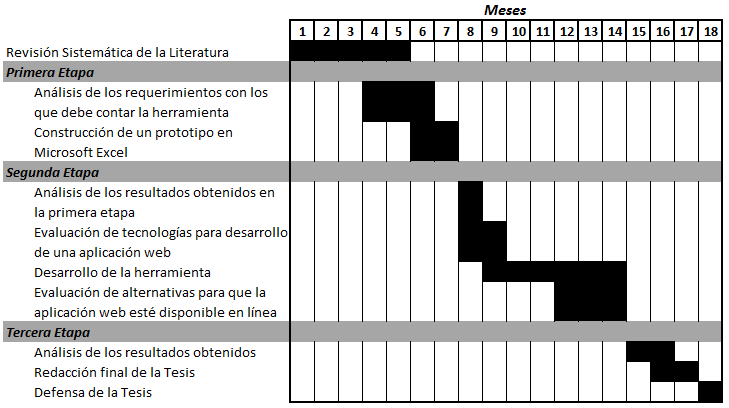
\includegraphics[width=1\linewidth,keepaspectratio]{./img/cronograma}
		\caption{Cronograma de trabajo}
		\label{fig:cronograma}
	\end{figure}
	
	% Referencias
		\printbibliography[category=cited]
		\printbibliography[title={Bibliograf�a},notcategory=cited]

\end{document}
